\chapter{Manual de Instalare 'si Utilizare}
\pagestyle{headings}

\section{Cerin'te}

'In acest capitol sunt prezentate cerin'tele software si hardware necesare compil'arii 'si utiliz'arii libr'ariei wxStyle.

\subsection{wxWidgets}

Pentru a compila 'si utiliza libr'aria wxStyle, trebuie s'a ave'ti la dispozi'tie fi'sierele binare redistribuite ale libr'ariei wxWidgets. Pute'ti ob'tine aceste fi'siere fie 'in urma compil'arii libr'ariei, fie desc'arc{\ia}nd de pe internet o versiune compilat'a a acesteia. At{\ia}t sursele libr'ariei c{\ia}t 'si versiunea compilat'a a acesteia pot fi downloadate gratuit de la adresa oficial'a\footnote{http://wxwidgets.org/downloads/}.

\subsection{boost}

Libr'aria boost pentru C++ poate fi downloadat'a gratuit de la adresa oficial'a\footnote{http://www.boost.org/users/download/}. Pute'ti alege sa downloada'ti fie sursele libr'ariei, fie o versiune precompilat'a. Dac'a alege'ti sa downloada'ti sursele, urma'ti pa'sii de instalare detalia'ti 'in documentul de utilizare al libr'ariei disponibil online\footnote{http://www.boost.org/doc/libs/1\_55\_0/more/getting\_started/}.

\subsection{Sistem de operare}

Pentru a func'tiona corect, wxStyle are nevoie de un sistem de operare pentru care wxWidgets s'a implementeze mecanismul avansat de desenare. Sistemele de operare suportate sunt: 
\begin{itemize}
\item \textbf{Windows:} Windows XP, Windows Vista, Windows 7, Windows 8, Windows 8.1 
\item \textbf{Unix:} Aproape toate implementarile Unix 'impreun'a cu un cel pu'tin un desktop manager la alegere dintre: GTK+ 1.2, GTK+ 2.0, Motif 1.2 sau mai nou, Lesstif.
\item \textbf{MacOS:} Mac OS 8.6/9.x (ex. Classic) sau Mac OS X 10.x. 
\end{itemize}

\subsection{Compilator}

Libr'aria wxStyle utilizeaz'a c{\ia}teva dintre noile adi'tii la standardul C++ introduse 'in versiunea numit'a C++11. Din acest motiv, compilarea libr'ariei necesit'a un compilator ce implementeaz'a aceste tr'as'aturi. Majoritatea compilatoarelor moderne implementeaz'a aproape 'in 'intregime standardul C++11 'si sunt potrivite pentru compilarea proiectului. Dintre acestea men'tion'am: Visual Studio 2012, Visual Studio 2013 'si gcc 4.9.0. Orice compilator a'ti alege, este recomandat'a folosirea celei mai noi versiuni pentru a asigura nu doar compatibilitatea cu standardul, dar 'si cele mai bune performan'te 'si securitate.

\section{Compilare 'si Instalare}

Toate fisierele necesare configur'arii 'si compil'arii proiectului se afl'a 'in folder-ul \texttt{build}. Pentru compilarea libr'ariei se folose'ste un mecanism automat de generare a fi'sierelor proiect pentru editorul integrat Visual Studio. Acestea se genereaz'a pe baza unui script lua numit \texttt{premale4.lua}, prin rularea script-ului bash \texttt{update\_build.bat}. 'Inainte de generarea proiectului, asigura'ti-v'a c'a fi'sierul \texttt{paths.lua} con'tine c'aile corecte c'atre libr'ariile wxWidgets 'si boost.

Fi'sierul \texttt{paths.lua} con'tine dou'a variabile ce trebuiesc asignate: \texttt{SYSTEM\_LIBS} 'si \texttt{BOOST\_LIBS}. La calea specificat'a de variabila \texttt{SYSTEM\_LIBS} trebuie s'a se g'aseasc'a dou'a foldere: 
\begin{itemize}
\item \texttt{include} care s'a con'tin'a con'tinutul folder-ul \texttt{include} din libr'aria wxWidgets
\item \texttt{lib} care s'a con'tin'a toate fi'sierele .lib compilate ale libr'ariei wxWidgets
\end{itemize}

Calea specificat'a de \texttt{SYSTEM\_LIBS} trebuie sa con'tin'a libr'aria boost compilat'a.

Pentru generarea proiectului Visual Studio, executati scriptul \texttt{update\_build.bat}. In urma execu'tiei trebuie s'a rezulte folder-ul \texttt{vc2012} ce con'tine, printre altele, proiectul \texttt{wxstyle.sln}. Deschide-'ti acest proiect in editorul integrat Visual Studio 2012. Proiectul ar trebui s'a arate similar cu cel din figura urm'atoare:

% =================================
% Figura Proiect Visual Studio
% =================================
\begin{figure}[H]
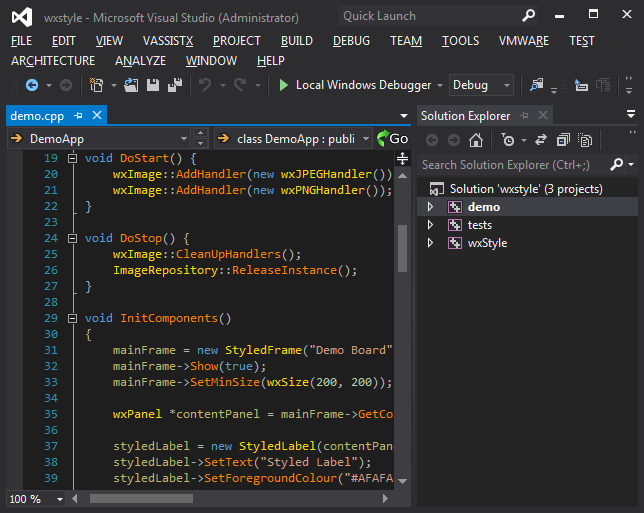
\includegraphics[width=15cm]{img/ch7_project.png}
\caption{Proiectul Visual Studio}
\label{fig:figure6.1}
\end{figure}

Pentru a compila libr'aria, este suficient s'a da'ti click dreapta pe numele proiectului wxStyle si alege'ti ac'tiunea Build. Proiectul este configurat sa compileze o librarie static'a, iar rezultatul compil'arii se poate gasi in folderul \texttt{lib}. Modul implicit de compilare este cel Debug, rezult{\ia}nd 'in libr'aria static'a \texttt{wxstyle\_d.lib} care con'tine 'si simboluri pentru depanare. Dac'a se alege din Visual Studio modul de compilare Release, rezultatul va fi \texttt{wxstyle.lib}.

Solu'tia con'tine de asemenea un proiect pentru testarea componentelor numit \texttt{tests} si un proiect demonstrativ ce prezint'a componentele libr'ariei wxStyle.


\section{Utilizare}

Aceast'a sec'tiune presupune c'a de'tine'ti o versiune compilat'a a libr'ariei dup'a ce a'ti urmat pa'sii din sec'tiunea anterioar'a. De asemenea, aceast'a sec'tiune presupune c'a ave'ti disponibil'a o versiune a editorului integrat Visual Studio 2012.

\subsection{Preg'atire}

Pentru a putea utiliza biblioteca wxStyle, trebuie s'a configura'ti 'in prealabil editorul Visual Studio 2012. Acest lucru presupune specificarea c'aii catre fi'sierele header ale bibliotecii, si a fisierului binar \emph{wxstyle.lib}.

\begin{enumerate}
\item Executa'ti click dreapta pe numele proiectului 'si alege'ti op'tiunea Properties.
\item La categoria \emph{C/C++}, subcategoria \emph{General} completa'ti c{\ia}mpul \emph{Additional Include Directories} cu calea relativ'a sau absolut'a c'atre folder-ul \emph{include} al bibliotecii wxStyle (vezi figura \ref{ch7_ide_include}).
\item La categoria \emph{Linker}, subcategoria \emph{General} completa'ti c{\ia}mpul \emph{Additional Library Directires} cu calea relativ'a sau absolut'a c'atre folder-ul \emph{lib} al bibliotecii wxStyle. In acest folder trebuie s'a existe fi'sierul compilat \emph{wxstyle.lib} (vezi figura \ref{ch7_ide_lib_folder})
\item La categoria \emph{Linker}, subcategoria \emph{Input} completa'ti c{\ia}mpul \emph{Additional Dependencies} cu numele fi'sierului binar al libr'ariei, mai exact \emph{wxstyle.lib} (vezi figura \ref{ch7_ide_lib_file}).
\end{enumerate}

\begin{figure}[H]
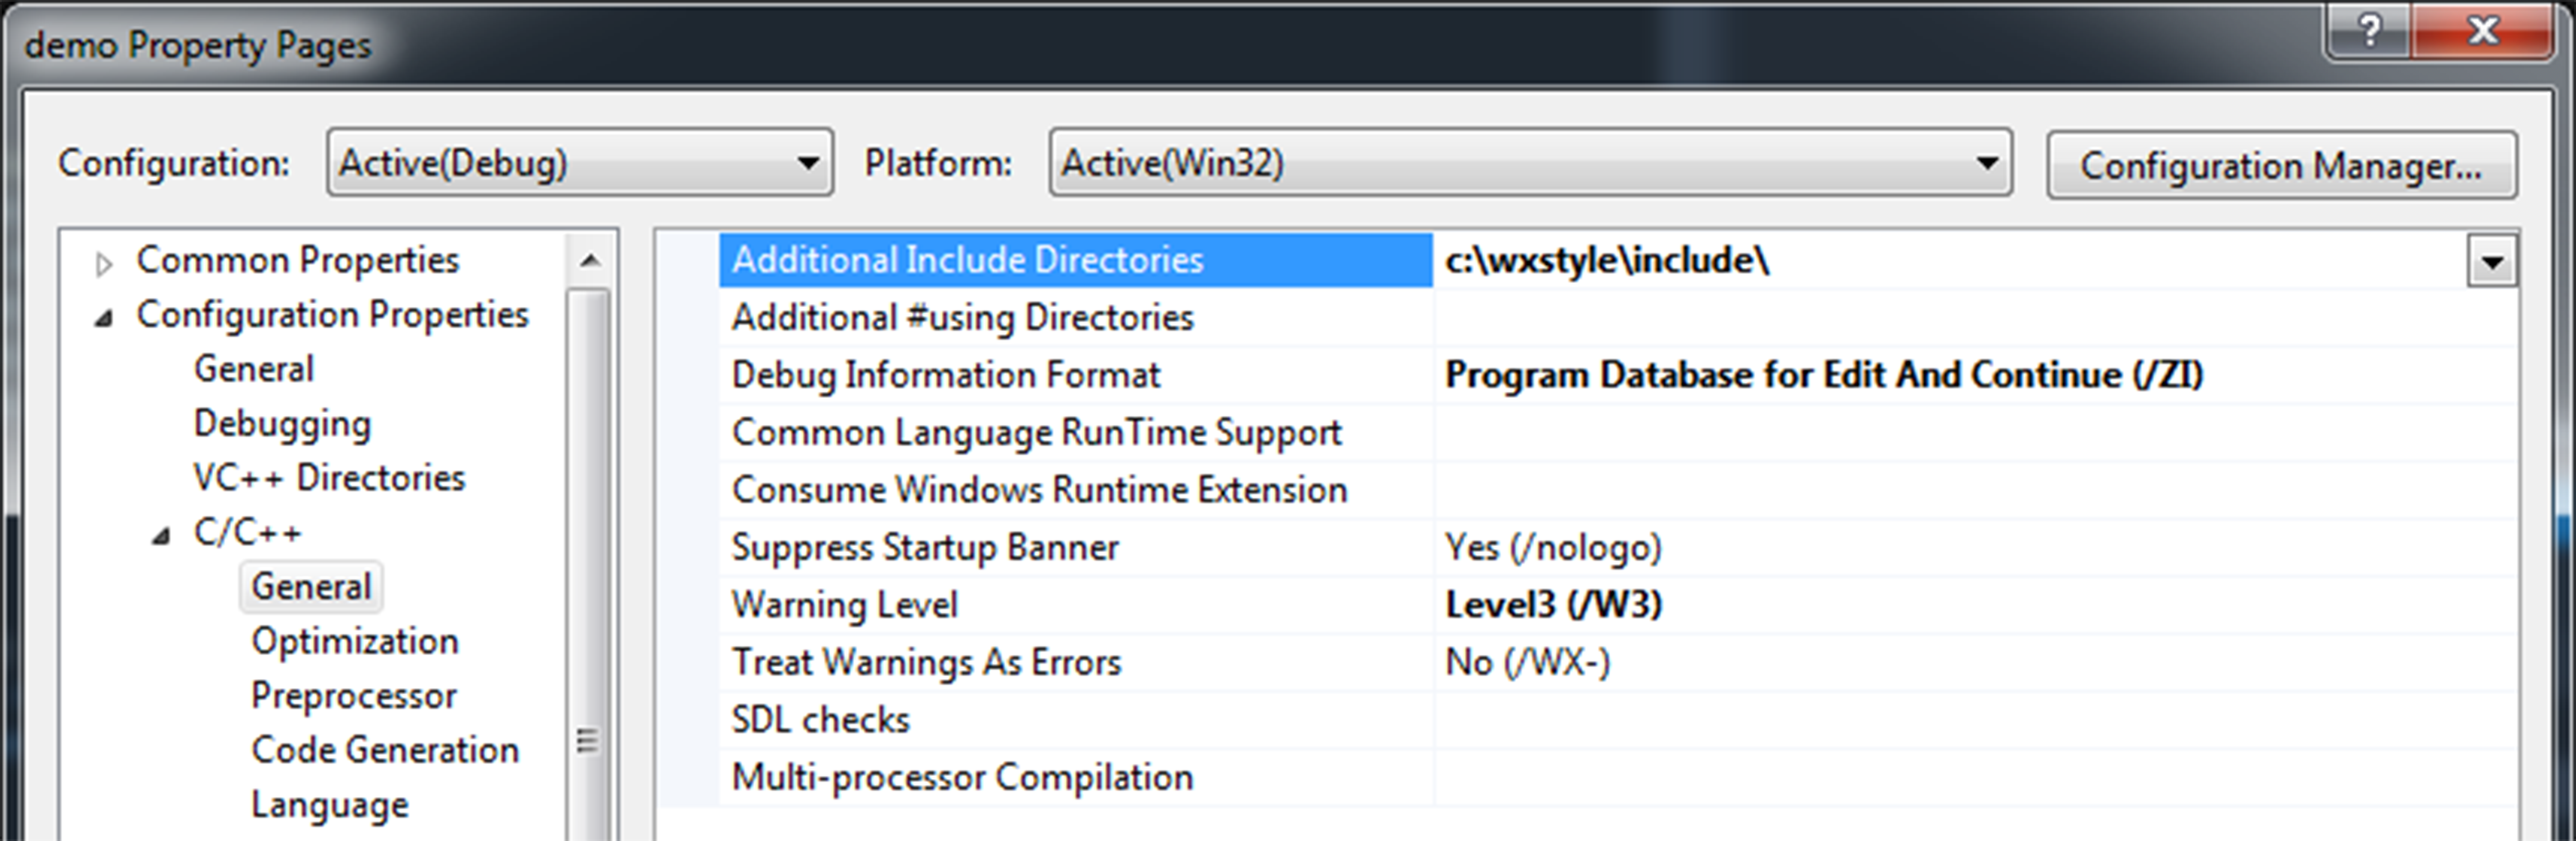
\includegraphics[width=15cm]{img/ch7_ide_include.png}
\caption{Setarea c'aii c'atre headerele bibliotecii wxStyle}
\label{ch7_ide_include}
\end{figure}

\begin{figure}[H]
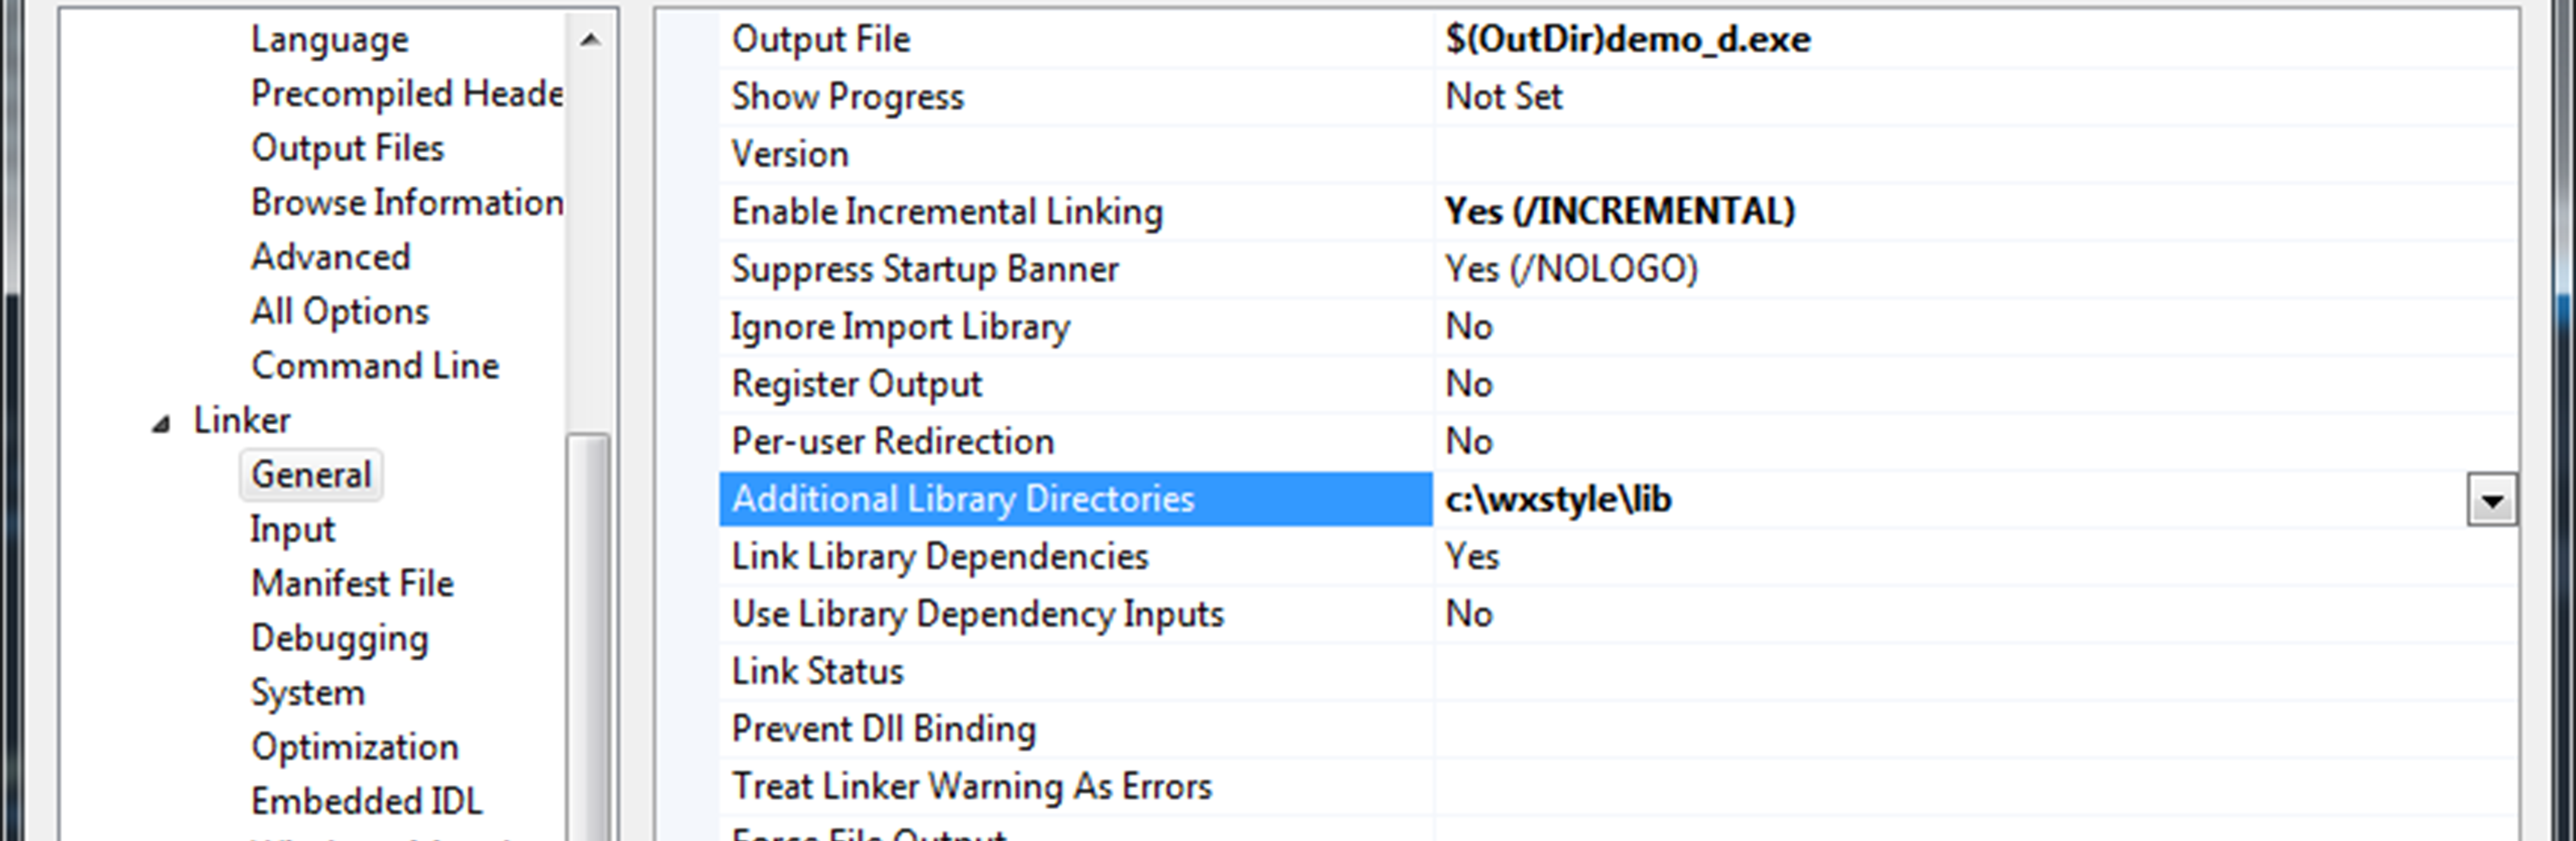
\includegraphics[width=15cm]{img/ch7_ide_lib_folder.png}
\caption{Setarea c'aii c'atre fi'sierul binar al bibliotecii wxStyle}
\label{ch7_ide_lib_folder}
\end{figure}

\begin{figure}[H]
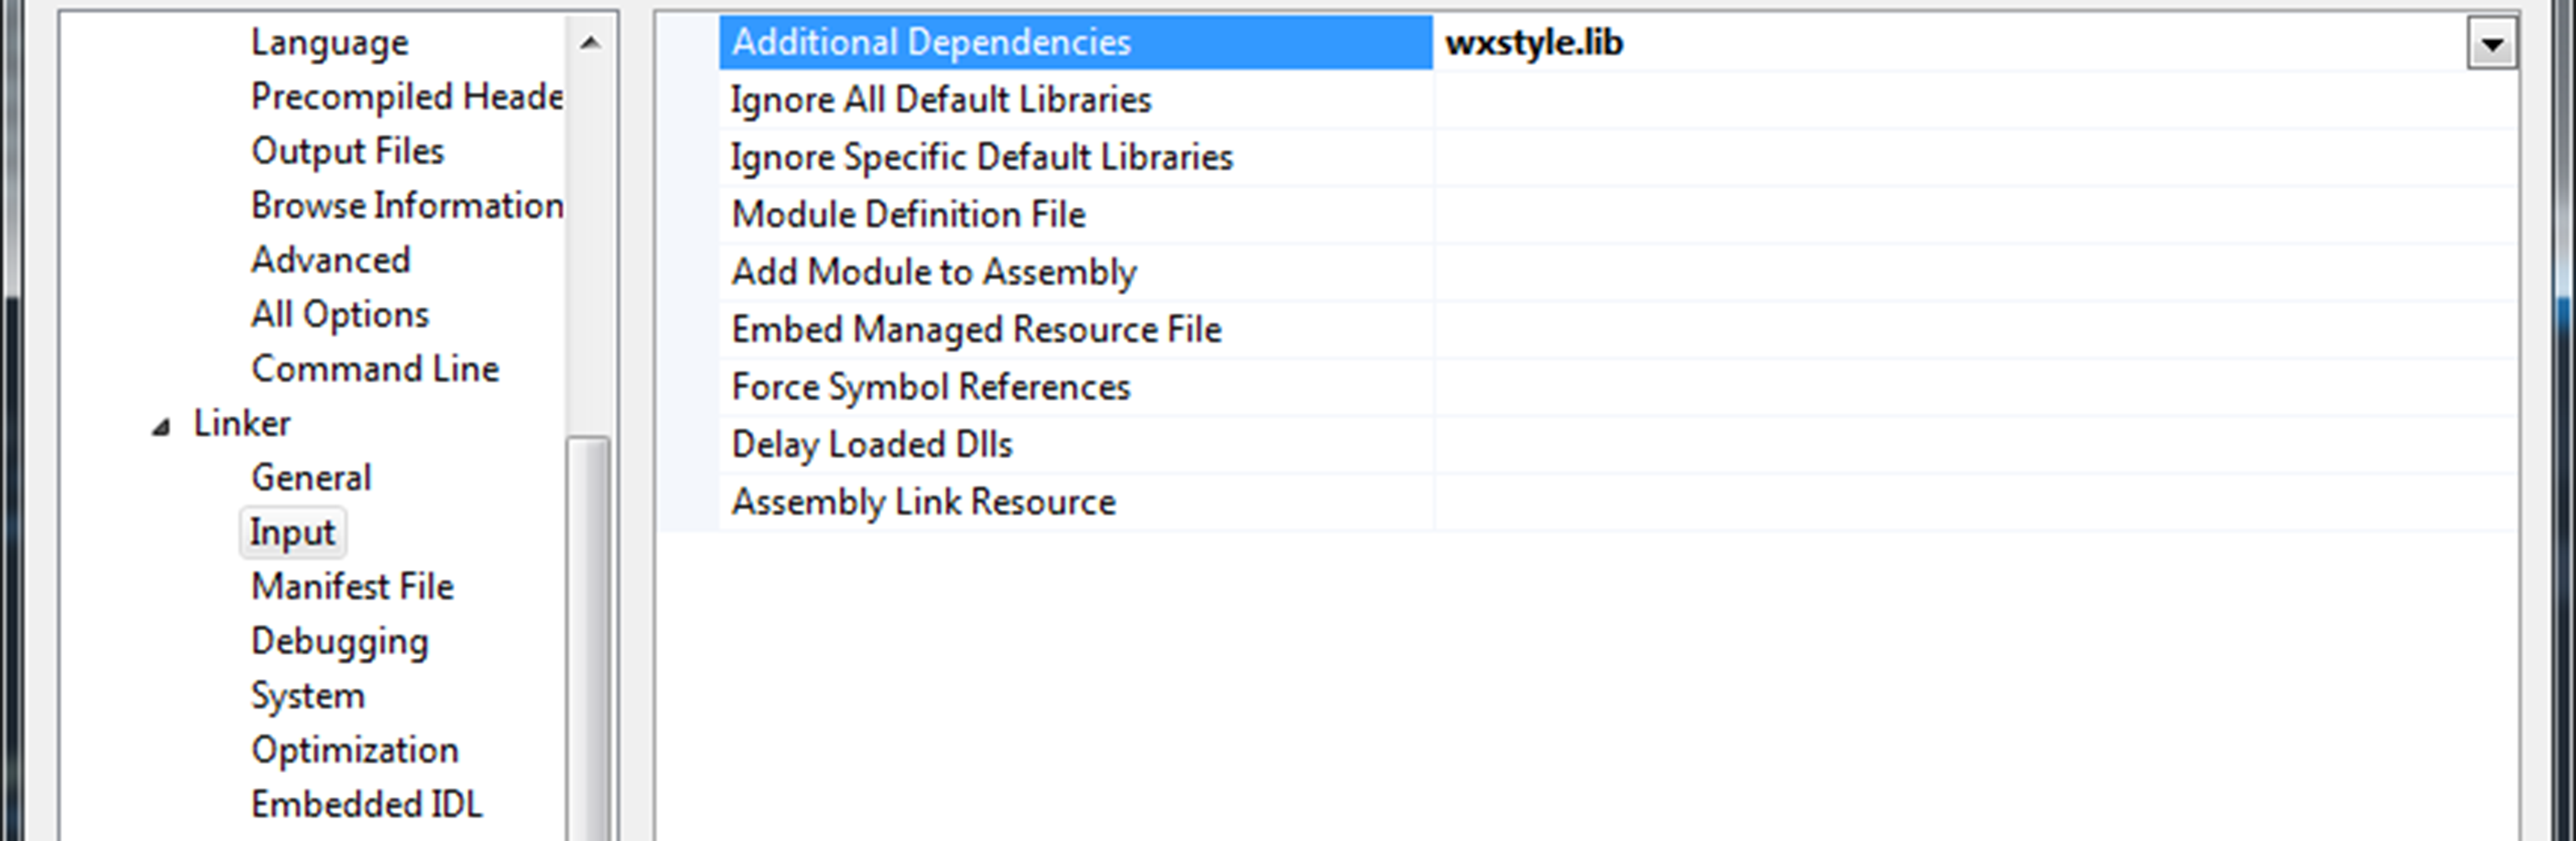
\includegraphics[width=15cm]{img/ch7_ide_lib_file.png}
\caption{Men'tionarea dependin'tei de fi'sierul binar wxstyle.lib}
\label{ch7_ide_lib_file}
\end{figure}

'In cele ce urmeaz'a, vom presupune c'a editorul Visual Studio 2012 recunoa'ste directivele de \emph{\#include} ce implic'a headere ale bibliotecii wxStyle, 'si g'ase'ste simbolurile compilate in fi'sierul binar wxstyle.lib

\subsection{Exemple de utilizare}

Scopul acestei sec'tiuni este de a prezenta sumar punctele de interes utiliz{\ia}nd exemple 'si explica'tii pentru cele mai des 'int{\ia}lnite situa'tii. Pentru informa'tii suplimentare, consulta'ti anexele A 'si B care prezint'a intreaga interfa't'a a bibliotecii si schema de descriere a limbajului utilizat la fi'sierele de stil. Mai ave'ti la dispozi'tie proiectul de prezentare numit \emph{demo} distribuit 'impreun'a cu aplica'tia.

\medskip

Din biblioteca \emph{wxStyle} pot fi folosite orice obiecte de interfa't'a oriunde 'in interiorul unei aplica'tii wxWidgets. Totu'si, este mai avantajoas'a folosirea unei ferestre stilizabile \emph{StyledFrame}. 'In interiorul acestei ferestre pot fi plasate at{\ia}t obiecte de interfa't'a wxWidgets c{\ia}t 'si componente stilizabile implementate in cadrul bibliotecii wxStyle. 'In plus fa't'a de ferestrele native implementate 'in wxWidgets, ferestrele stilizabile pot fi modificate 'in orice mod, de la schimbarea componentelor ce alc'atuiesc titlul ferestrei p{\ia}n'a la schimbarea fundalului cu o imagine transparent'a. Un exemplu ce construie'ste o fereastr'a \emph{StyledFrame} este prezentat 'in figura \ref{ex01}.

\begin{figure}[H]
\begin{lstlisting}[language=C++]
#include "StyledFrame.h"
using namespace wxstyle;
StyledFrame* CreateStyledFrame() {
	StyledFrame frame = new StyledFrame("Demo Board");
	frame->SetMinSize(wxSize(200, 200));
	frame->Show(true);
	return frame;
}
\end{lstlisting}
\caption{Exemplu de construire a unei ferestre \emph{StyledFrame}}
\label{ex01}
\end{figure}

Obiectele de interfa't'a se construiesc in mod similar celor implementate in wxWidgets, cu excep'tia faptului c'a acestea nu necesit'a asocierea unui identificator unic. Toate obiectele de interfa't'a au 'in comun un constructor ce specific'a obiectul p'arinte 'si textul obiectului (parametru op'tional). 'In cele mai multe situa'tii, p'arintele unui obiect va fi panoul de con'tinut al ferestrei care 'il con'tine. Exemplul din figura \ref{ex02} demonstreaz'a procesul de construire al unor obiecte de interfa't'a. Pozi'tionarea obiectelor 'in interiorul ferestrei se face folosind un obiect \emph{wxSizer} ata'sat panoului de con'tinut al ferestrei, a'sa cum se procedeaz'a 'in cadrul libr'ariei wxWidgets.

\begin{figure}[H]
\begin{lstlisting}[language=C++]
#include "StyledFrame.h"
#include "StyledLabel.h"
#Include "StyledButton.h"
using namespace wxstyle;
void CreateUIObjects(StyledFrame *frame) {
	wxPanel *contentPanel = frame->GetContentPanel();
	StyledLabel *label = new StyledLabel(contentPanel, "some text");
	StyledButton *button = new StyledButton(contentPanel, "some action");
}
\end{lstlisting}
\caption{Exemplu de construire al unor obiecte de interfa't'a}
\label{ex02}
\end{figure}

Stilizarea obiectelor de interfa't'a se face utiliz{\ia}nd structuri de tipul \emph{Style}. Acestea con'tin informa'tii necesare prezent'arii obiectelor 'in st'arile principale ale acestora: \emph{default}, \emph{disabled}, \emph{focused}, \emph{hovered}, \emph{pressed}. Un exemplu ce construie'ste un obiect de stil este prezentat in figura \ref{ex03}

\begin{figure}[H]
\begin{lstlisting}[language=C++]
#include "style/Style.h"
using namespace wxstyle;
Style* CreateStyle() {
	Style *result = new Style();
	DefinitionBundle bundle;
	bundle.SetFont(FontDefinition().SetFace("Tahoma").SetSize(3));
	bundle.SetForeground("#A2A2A2");
	bundle.SetOpaque(true);
	result.AddBundle(Style::CAT_DEFAULT, bundle);
	return result;
}
\end{lstlisting}
\caption{Exemplu de construire a unui stil}
\label{ex03}
\end{figure}

Defini'tiile necesare prezent'arii unui obiect sunt definite prin structuri precum \emph{FontDefinition}, \emph{ShadowDefinition} sau valori simple precum \emph{wxColour}. Acestea sunt agregate de structuri \emph{DefinitionBundle}. O astfel de structur'a este ata'sat'a unui stil la o categorie ce reprezint'a una din starile fundamentale ale unui obiect de interfa't'a.

\medskip

Deoarece construirea stilurilor prin cod este complicat'a, anevoioas'a 'si rigid'a, stilurile pot fi specificate prin fi'siere de stil numite \emph{stylesheets}. Acestea respect'a o structur'a clar'a, descris'a de schema XST prezent'a 'in Anexa A. Un exemplu de astfel de fi'sier este prezent 'in figura \ref{ex04}

\begin{figure}[H]
\begin{lstlisting}[language=XML]
<stylesheet name="test">
  <styles>
    <style name="default">
	  <default>
	    <font face="Tahoma" size="3"/>
		<insets rect="10, 3, 5, 3"/>
		<foreground color="#A2A2A2"/>
		<opacity value="true"/>
	  </default>
	</style>
  </styles>
</stylesheet>
\end{lstlisting}
\caption{Exemplu de fi'sier \emph{stylesheet}}
\label{ex04}
\end{figure}

Pentru a aduce 'in memorie stilurile con'tinute 'intr-un fi'sier de stiluri, se poate utiliza clasa \emph{XMLStylesheetLoader}. Rezultatul pars'arii unui astfel de fi'sier este o structur'a numit'a \emph{Stylesheet} ce con'tine o map'a de la numele unui stil la structura de stil. Un exemplu de astfel de parsare se g'ase'ste in figura \ref{ex05}

\begin{figure}[H]
\begin{lstlisting}[language=C++]
#include <string>
#include "style/XMLStylesheetLoader.h"
using namespace wxstyle;
void LoadStylesheet(const std::string& file) {
	XMLStylesheetLoader loader;
	Stylesheet stylesheet = loader.Load(file);
	Style defaultStyle = stylesheet.GetStyle("default");
}
\end{lstlisting}
\caption{Exemplu de parsarea a unui fi'sier de stiluri folosind \emph{XMLStylesheetLoader}}
\label{ex05}
\end{figure}

Asignarea unui stil la un obiect de interfa't'a se face utiliz{\ia}nd metoda \emph{SetStyle}. De asemenea, metoda \emph{GetStyle} este utilizat'a pentru ob'tinerea stilului asociat. Pentru extragerea structurii de tip \emph{StyleBundle} asociate unui obiect 'si care este corespunz'atoare st'arii acestuia se folose'ste metoda \emph{GetDefinitionBundle}. Aceast'a methoda combin'a bundle-ul default cu bundle-ul asociat st'arii pentru a genera un bundle gata de folosit. Un exemplu de utilizare al acestor metode se g'ase'ste in figura \ref{ex06}.

\begin{figure}[H]
\begin{lstlisting}[language=C++]
#include "style/Style.h"
#include "style/DefinitionBundle.h"
#include "StyledLabel.h"
using namespace wxstyle;
void SetStyleExample(const StyledLabel& label, const Style& style) {
	label.SetStyle(style);
	DefinitionBundle bundle = label.GetDefinitionBundle();
}
\end{lstlisting}
\caption{Exemplu de setarea a stilului unui obiect 'si extragerea unui \emph{DefinitionBundle}}
\label{ex06}
\end{figure}

Procesarea de evenimente se face diferit c{\ia}nd vine vorba de obiectele de interac'tiune ale bibliotecii wxStyle. Pentru ata'sarea unei metode de procesare unui eveniment utiliz'am obiecte de tipul listener asociate fiec'arei categorii de evenimente. Figura \ref{ex07} exemplific'a acest mecanism.

\begin{figure}[H]
\begin{lstlisting}[language=C++]
#include "StyledWindow.h"
using namespace wxstyle;
class ExampleMouseListener : public StyledWindow::MouseListener {
public:
	void MouseDown(const wxMouseEvent& mouseEvent) override {
		// Process the mouse event
	}
};
void RegisterEvent(const StyledWindow& window) {
	window->RegisterMouseListener(new ExampleMouseListener());
}
\end{lstlisting}
\caption{Exemplu de procesarea al evenimentelor generate de dispozitiv-ul mouse folosind obiecte de tip \emph{MouseListener}}
\label{ex07}
\end{figure}

Exemplele prezentate in aceast'a sec'tiune nu fac dec{\ia}t sa acopere suprafa'ta bibliotecii wxStyle. Posibilit'a'tile de stilizare 'si compunere a obiectelor de interfa't'a sunt nenum'arate. Pentru o documenta'tie complet'a, consulta'ti anexele A 'si B ce descriu 'in 'intregime formatul fi'sierelor de stiluri 'si a componentelor bibliotecii.